\RequirePackage{luatex85}
\documentclass{standalone}

% Default preamble
\usepackage{pgfplots}
\usepackage{tikz}
\usetikzlibrary{%
    patterns, plotmarks, backgrounds, shapes, arrows, calc, trees, positioning,
    chains, shapes.geometric, decorations.pathreplacing,
    decorations.pathmorphing, shapes.arrows, decorations.markings, quotes,
    arrows.meta, spy, fit, matrix, math
}

% Custom preamble from global variable:
\usetikzlibrary{patterns}
\usepackage{xcolor}
\definecolor{efm1}{HTML}{017EC3}
\definecolor{efm2}{HTML}{F31E26}
\definecolor{efm3}{HTML}{019E5E}
\definecolor{efm4}{HTML}{FBA61D}
\definecolor{efm5}{HTML}{916237}

\usepackage{graphicx}
\usepackage{caption}
\usepackage{subcaption}
\usepackage{amsmath}

\renewcommand{\familydefault}{\sfdefault}

\begin{document}

\begin{figure}
    \begin{tikzpicture}
        \node[] (start) {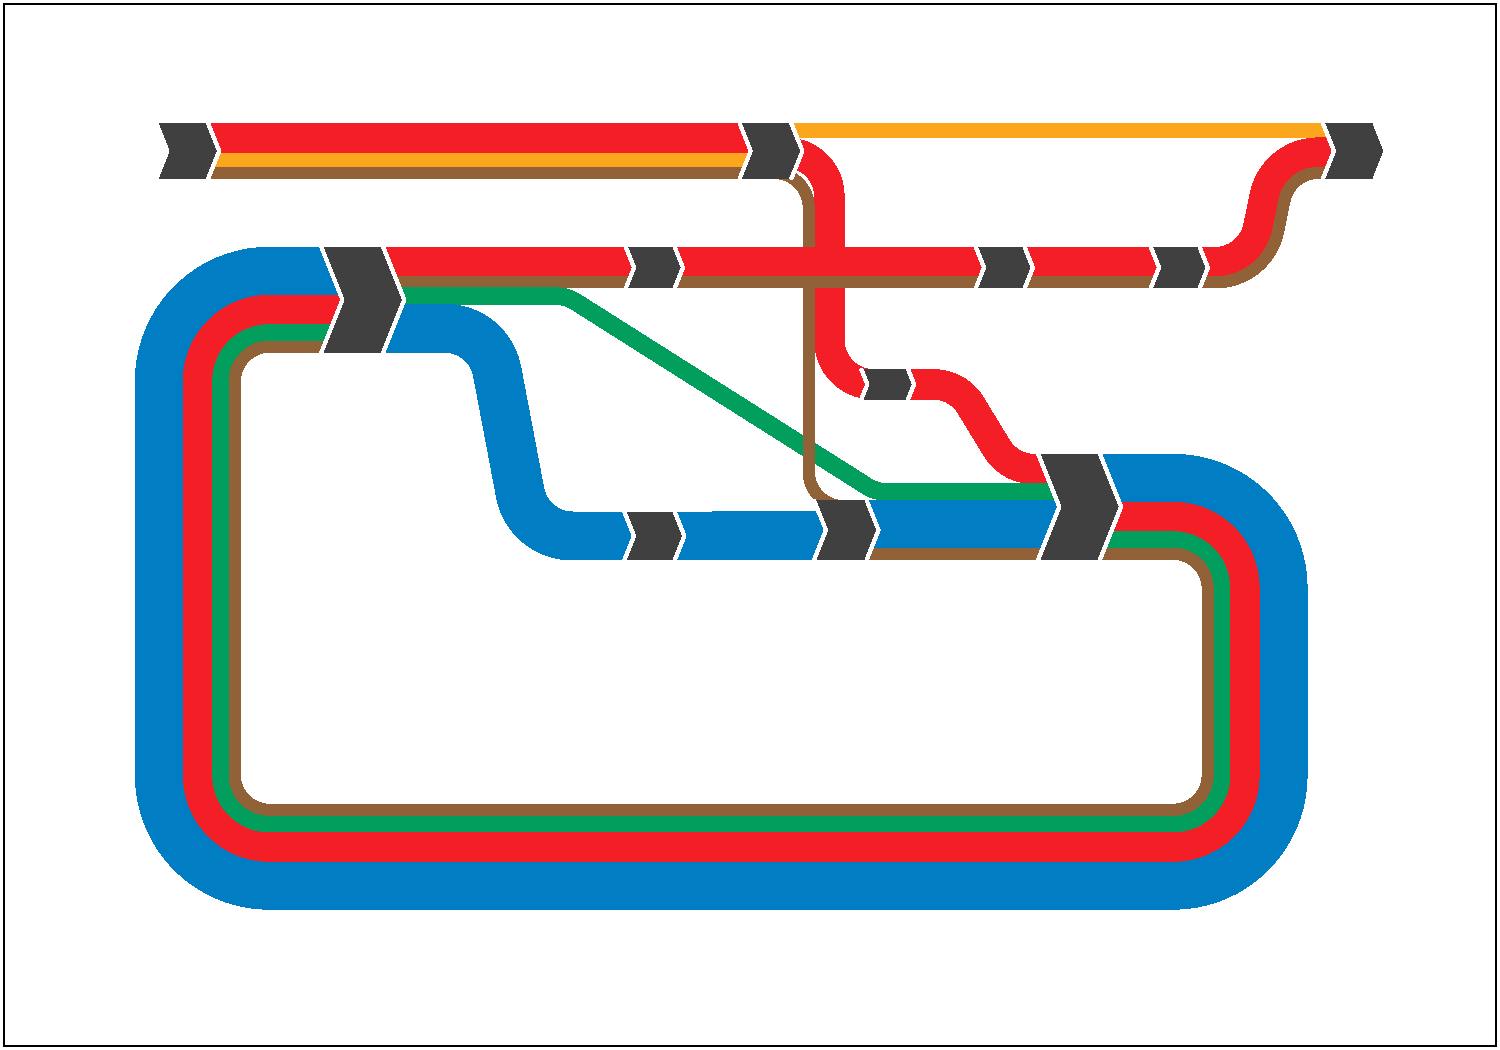
\includegraphics[width=0.85\textwidth,trim={1.75cm 0.25cm 1.5cm 0.25cm},clip]{../02-R-output-figures/sankey-unlabelled.pdf}};
        \node[above=0.1cm of start] () {};
        \node[below=1.45cm of start] () {};
    \end{tikzpicture}
\end{figure}

\end{document}

